\documentclass[a4paper,11pt]{article}

\usepackage[utf8]{inputenc}
\title{ARC1 - TP 1}
\author{Léo Noël-Baron \& Thierry Sampaio}
\date{02/10/2015}

\usepackage{a4wide}
\usepackage{textcomp}
\usepackage[utf8]{inputenc}
\usepackage[T1]{fontenc}
\usepackage[francais]{babel}

\usepackage{graphicx}
\usepackage[usenames,dvipsnames]{color}

\usepackage{hyperref} \urlstyle{sf}
\hypersetup{
  colorlinks=true,
  urlcolor=BlueViolet,
  citecolor=BlueViolet,
  linkcolor=BlueViolet,
}
\DeclareUrlCommand\email{\urlstyle{sf}}

\newenvironment{keywords}
  {\description\item[\bsc{Mots-clés}]~$\cdot$~ }
  {\enddescription}
\newenvironment{remarque}
  {\description\item[\bsc{Remarque} ---]\sl}
  {\enddescription}
\renewcommand{\thefootnote}{\arabic{footnote}}

\usepackage{listings}
\lstset{
  language=C,
  basicstyle=\ttfamily,
  keywordstyle=\color{OliveGreen},
  stringstyle=\color{Bittersweet},
  showstringspaces=false,
  commentstyle=\color{Gray},
  numbers=left,
  numberstyle=\ttfamily\color{Gray},
  frame=l,
  columns=fullflexible,
  rulecolor=\color{Gray},
  tabsize=4,
  extendedchars=true,
  literate=
	{É}{{\'E}}1 {è}{{\`e}}1 {à}{{\`a}}1 {È}{{\`E}}1 {À}{{\`A}}1 {ê}{{\^e}}1 {â}{{\^a}}1 {î}{{\^\i}}1 {ô}{{\^o}}1
	{Ê}{{\^E}}1 {Â}{{\^A}}1 {Î}{{\^I}}1 {Ô}{{\^O}}1 {Û}{{\^U}}1 {ë}{{\"e}}1 {ï}{{\"\i}}1 {ü}{{\"u}}1 {Ë}{{\"E}}1
	{Ï}{{\"I}}1 {Ü}{{\"U}}1 {û}{{\^u}}1 {ç}{{\c c}}1 {Ç}{{\c C}}1 {æ}{{\ae}}1 {Æ}{{\AE}}1 {œ}{{\oe}}1 {Œ}{{\OE}}1
	{é}{{\'e}}1,
}
\lstMakeShortInline{|}

\parskip=0.3\baselineskip
\sloppy

\makeatletter
  \let\runtitle\@title
  \let\runauthor\@author
\makeatother

\usepackage{fancyhdr}
\pagestyle{fancy}
\fancyhead{}
\lhead{\runtitle}
\rhead{\runauthor}
\setlength{\headheight}{13.6pt}


\begin{document}

\maketitle

\subsection*{Porte OU}

Le théorème de De Morgan donne $A+B = \overline{\overline{A+B}} = \overline{\overline{A}\cdot\overline{B}}$, ce qui permet facilement de construire une porte OU (Figure \ref{nandor}) avec trois portes NON-ET, deux d'entre elles étant utilisées pour faire la négation de $A$ et de $B$.

\begin{figure}
\center
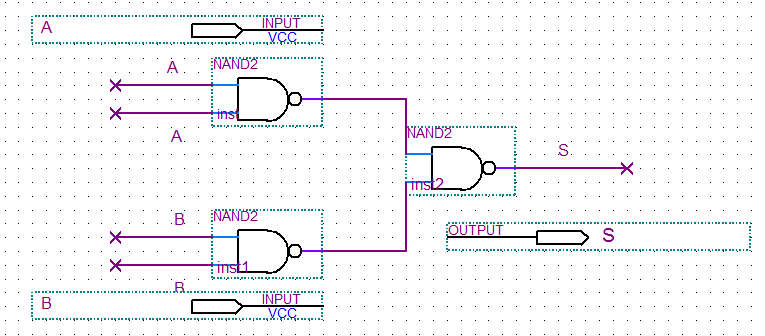
\includegraphics[scale=0.6]{nandor.png}
\caption{Schéma de circuit d'une porte OU}
\label{nandor}
\end{figure}

\subsection*{Regroupement de fils}

Pour ce circuit, il suffit de relier des bus d'entrées et de sortie de 4 bits au composant ADD4 existant, ce qui donne le schéma en Figure \ref{add4group}.

\begin{figure}
\center
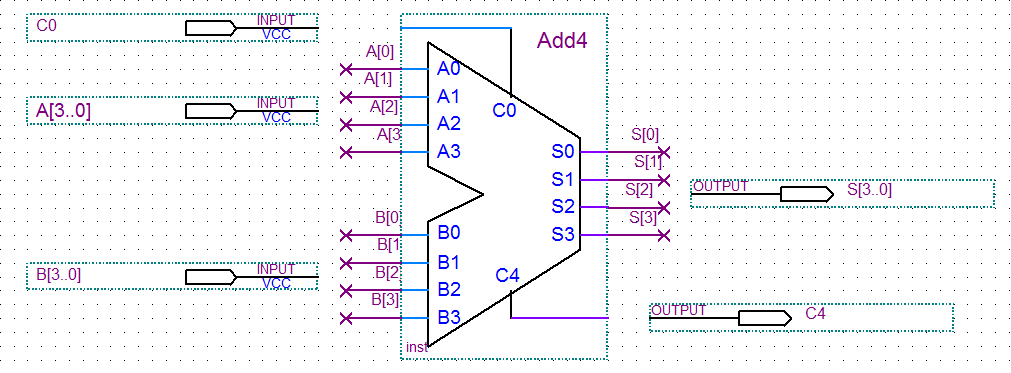
\includegraphics[scale=0.58]{add4.png}
\caption{Schéma de circuit du composant ADD4GROUP}
\label{add4group}
\end{figure}

\subsection*{Sélection par 3-états}

1. La définition de ce composant donne immédiatement le schéma de la Figure \ref{sel4}.
\begin{figure}
\center
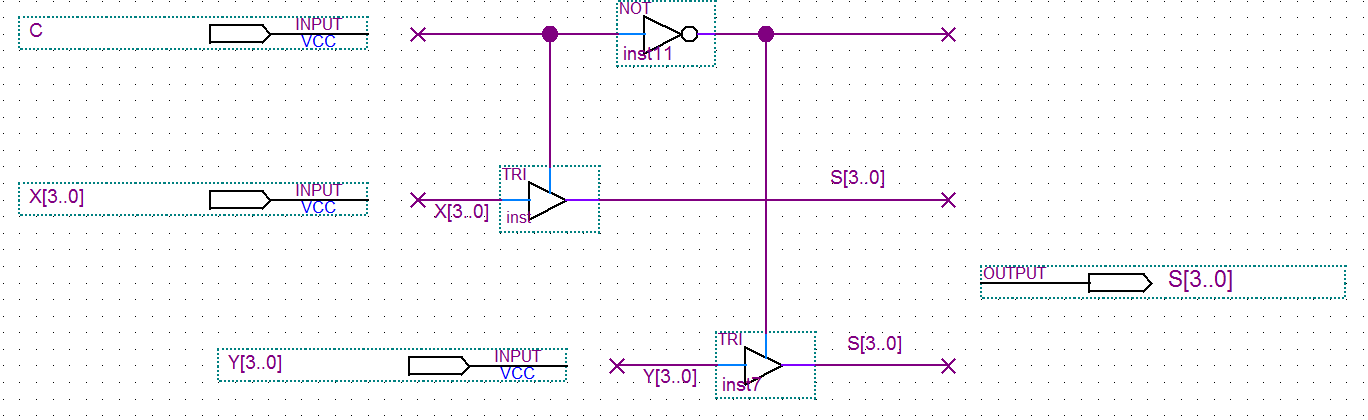
\includegraphics[scale=0.43]{sel4.png}
\caption{Schéma de circuit du composant SEL4}
\label{sel4}
\end{figure}

2. On choisit de prendre les deux opérandes $X$ et $Y$ depuis les interrupteurs 17 à 10, et la commande $C$ depuis l'interrupteur 9. Le composant ADD4GROUP permet de réaliser l'addition modulo 16 ; il suffit donc de le rediriger, ainsi que $X$, dans le SEL4 dont la sortie sera affichée sur les diodes rouges 17 à 14. Le circuit obtenu est présenté en Figure \ref{circuit}.
\begin{figure}
\center
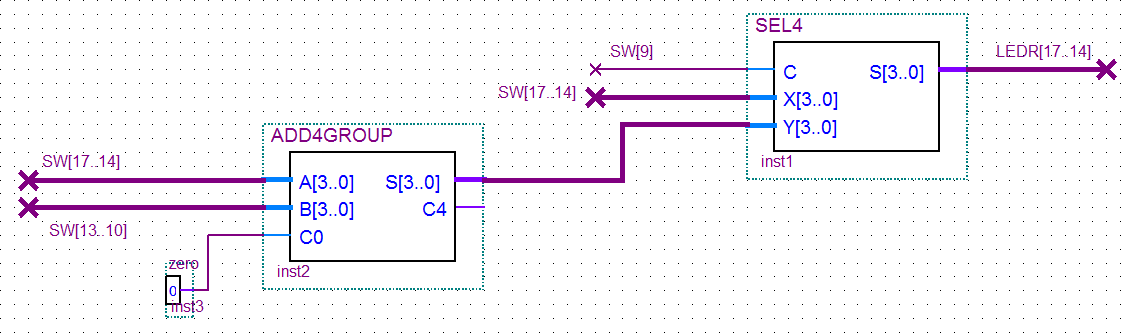
\includegraphics[scale=0.52]{final.png}
\caption{Schéma du circuit final}
\label{circuit}
\end{figure}

\end{document}
